\chapter{Web cache as an application}
\label{chap:webcache}

All applications described above are ``virtual'' applications, in the sense
that they do not actually transfer their own data in the simulator; all 
that matter is the \emph{size} and the \emph{time} when data are transferred.
Sometimes we may want applications to transfer their own data in simulations.
One such example is web caching, where we want HTTP servers to send HTTP 
headers to caches and clients. These headers contain 
page modification time information and other caching directives, which are 
important for some cache consistency algorithms.

In the following, we first describe general issues regarding
transmitting application-level data in \ns, then we discuss special
issues, as well as APIs, related to transmitting application data
using TCP as transport. We will then proceed to discuss the internal
design of HTTP client, server, and proxy cache. 

\section{Using application-level data in \ns}

\begin{figure}[tb]
  \begin{center}
    \centerline{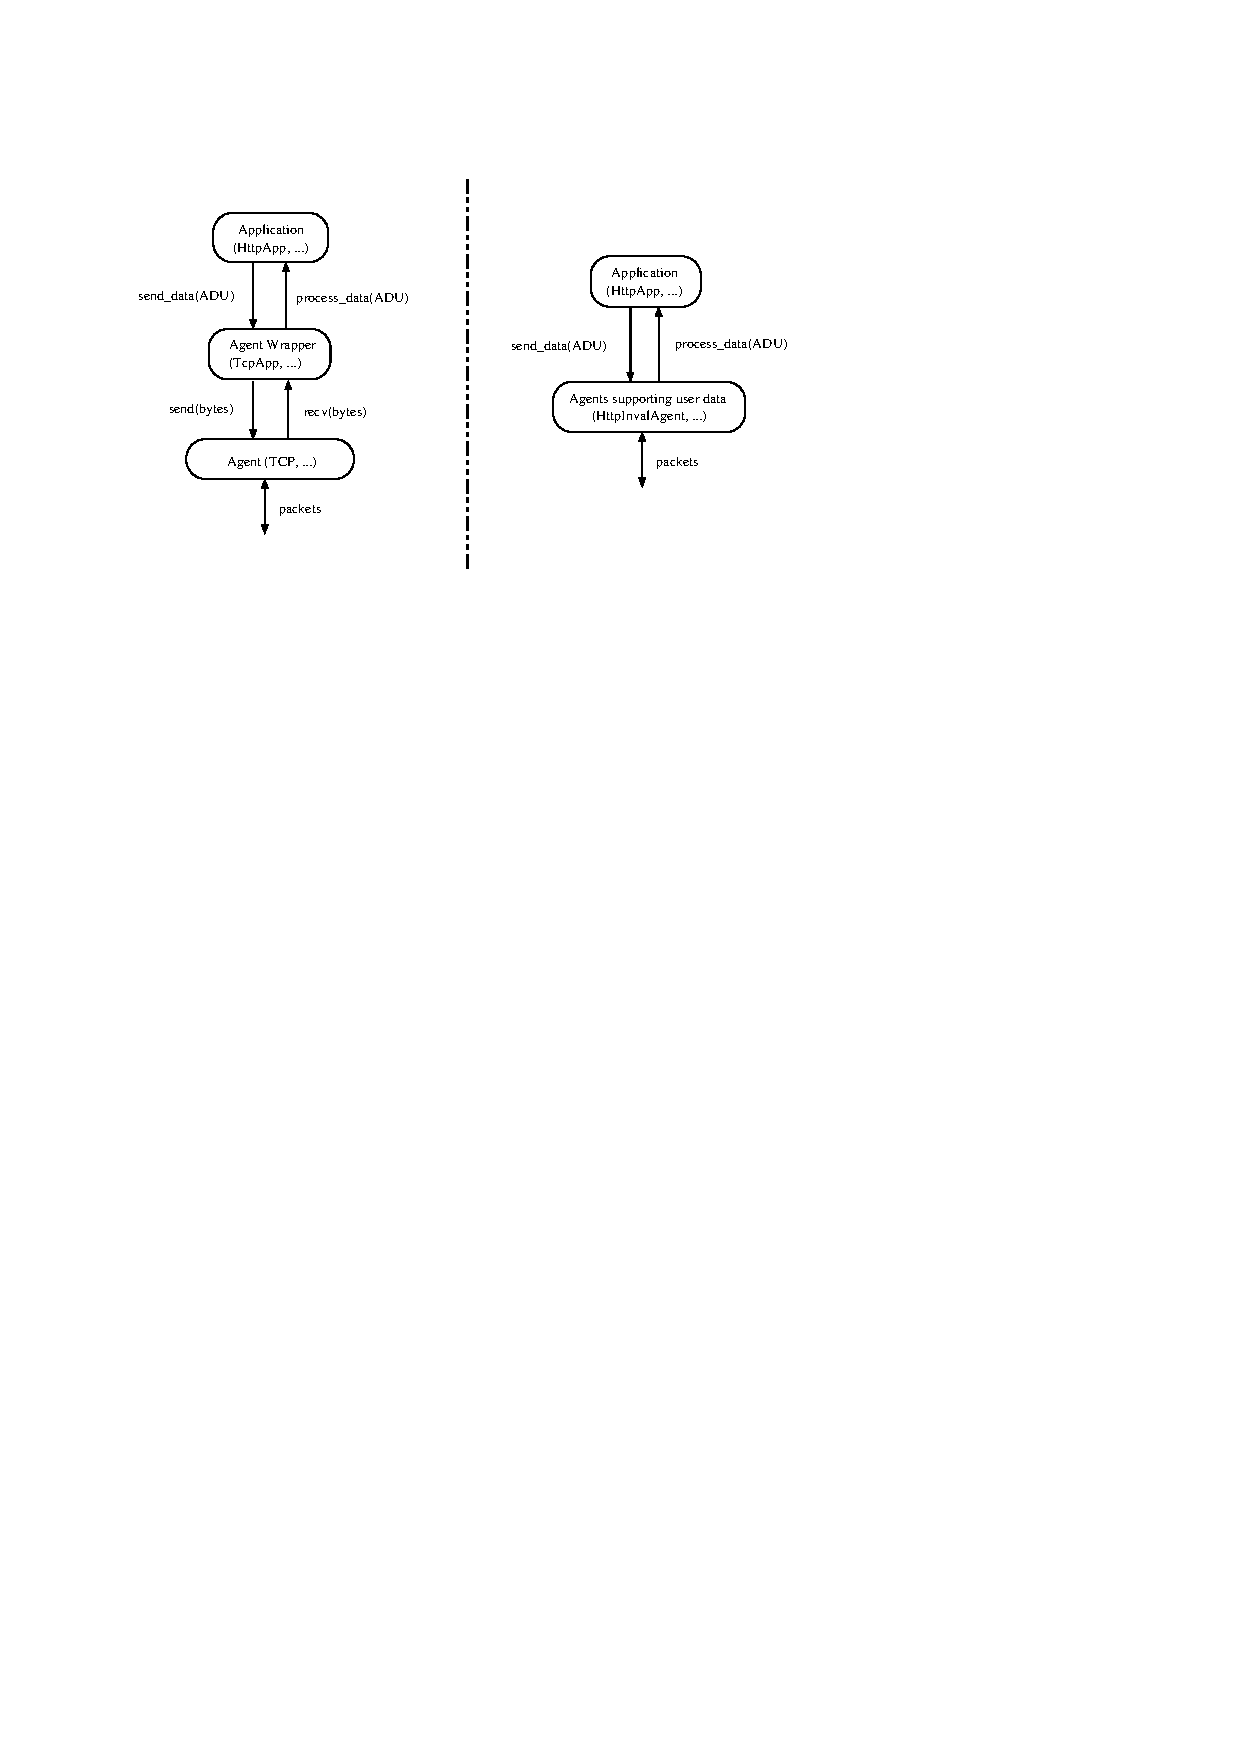
\includegraphics{app-dataflow}}
    \caption{Examples of application-level data flow}
    \label{fig:app-dataflow}
  \end{center}
\end{figure}

In order to transmit application-level data in \ns, we provide a 
uniform structure to pass data among applications, and to
pass data from applications to transport agents (Figure
\ref{fig:app-dataflow}). It has three major components: 
a representation of a uniform application-level data unit (ADU), a 
common interface to pass data between applications, and two mechanisms
to pass data between applications and transport agents.

\subsection{ADU} 

The functionality of an ADU is similar to that of a Packet. It needs to
pack user data into an array, which is then included in the user data
area of an \ns packet by an Agent (this is not supported by current
Agents. User must derive new agents to accept user data from
applications, or use an wrapper like TcpApp. We'll discuss this
later). 

Compared with Packet, ADU provides this functionality in a different
way. In Packet, a common area is allocated for all packet headers; an
offset is used to access different headers in this area. In ADU this
is not applicable, because some ADU allocates their space dynamically
according the the availability of user data. For example, if we want
to deliver an OTcl script between applications, the size of the script
is undetermined beforehand. Therefore, we choose a less efficient but
more flexible method. Each ADU defines its own data members, and
provides methods to serialize them (i.e., pack data into an array and
extract them from an array). For example, in the abstract base class
of all ADU, AppData, we have:

\begin{program}
        class AppData \{
        private:
                AppDataType type_;  // ADU type
        public:
                struct hdr \{
                        AppDataType type_;
                \};
        public:
                AppData(char* b) \{
                        assert(b != NULL);
                        type_ = ((hdr *)b)->type_;
                \}
                virtual void pack(char* buf) const;
        \}
\end{program}

Here \code{pack(char* buf)} is used to write an AppData object
into an array, and \code{AppData(char* b)} is used to build a new
AppData from a ``serialized'' copy of the object in an array.

When deriving new ADU from the base class, users may add more data,
but at the same time a new \code{pack(char *b)} and a new constructor 
should be provided to write and read those new data members from an
array. For an example as how to derive from an ADU, look at 
\ns/webcache/http-aux.h.

\subsection{Passing data between applications}

The base class of Application, Process, allows applications to pass
data or request data between each other. It is defined as follows:
\begin{program}
        class Process \{
        public: 
                Process() : target_(0) \{\}
                inline Process*& target() \{ return target_; \}

                virtual void process_data(int size, char* data) = 0;
                virtual void send_data(int size, char* data = 0);

        protected:
                Process* target_;
        \};
\end{program}

Process enables Application to link together. 
%{\bf TBA}

\subsection{Transmitting user data over UDP}

Currently there is no support in class Agent to transmit user
data. There are two ways to transmit a serialized ADU through transport
agents. First, for UDP agent (and all agents derived from there), we
can derive from class UDP and add a new method
\code{send(int nbytes, char *userdata)} to pass user data from
Application to Agent. To pass data from an Agent to an Application is
somewhat trickier: each agent has a pointer to its attached
application, we dynamically cast this pointer to an AppConnector and
then call \code{AppConnector::process_data()}.

As an example, we illustrate how class HttpInvalAgent is
implemented. It is based on UDP, and is intended to deliver web cache
invalidation messages (\ns/webcache/inval-agent.h). It is defined as:

\begin{program}
        class HttpInvalAgent : public Agent \{
        public: 
                HttpInvalAgent();

                virtual void recv(Packet *, Handler *);
                virtual void send(int realsize, AppData* data);

        protected:
                int off_inv_;
        \};
\end{program}

Here \code{recv(Packet*, Handler*)} overridden to extract user data,
and a new \code{send(int, AppData*)} is provided to include user data
in packetes. An application (HttpApp) is attached to an HttpInvalAgent
using \code{Agent::attachApp()} (a dynamic cast is needed). In
\code{send()}, the following code is used to write user data from
AppData to the user data area in a packet:

\begin{program}
        Packet *pkt = allocpkt(data->size());
        hdr_inval *ih = (hdr_inval *)pkt->access(off_inv_);
        ih->size() = data->size();
        char *p = (char *)pkt->accessdata();
        data->pack(p);
\end{program}

In \code{recv()}, the following code is used to read user data from
packet and to deliver to the attached application:

\begin{program}
        hdr_inval *ih = (hdr_inval *)pkt->access(off_inv_);
        ((HttpApp*)app_)->process_data(ih->size(), (char *)pkt->accessdata());
        Packet::free(pkt);
\end{program}


\subsection{Transmitting user data over TCP}
\label{sec:webcache-tcpapp}

Transmitting user data using TCP is trickier than doing that over UDP,
mainly because of TCP's reassembly queue is only available for
FullTcp. We deal with this problem by abstracting a TCP connection as
a FIFO pipe. 

As indicated in section \ref{sec:upcalls}, transmission of application data
can be implemented via agent upcalls. Assuming we are using TCP agents, 
all data are delivered in sequence, which means we can view the TCP 
connection as a FIFO pipe. We emulate user data transmission over TCP
as follows. We first provide buffer 
for application data at the sender. Then we count the bytes received at the 
receiver. When the receiver has got all bytes of the current data transmission,
it then gets the data directly from the sender. Class Application/TcpApp is 
used to implement this functionality.

A TcpApp object contains a pointer to a transport agent, presumably either
a FullTcp or a SimpleTcp.
\footnote{A SimpleTcp agent is used solely for web caching simulations. It 
is actually an UDP agent. It has neither error recovery nor flow/congestion
control. It doesn't do packet segmentation. Assuming a loss-free network 
and in-order packet delivery,
SimpleTcp agent simplifies the trace files 
and hence aids the debugging of application protocols, which, in our case, 
is the web cache consistency protocol.}
(Currently TcpApp doesn't support asymmetric TCP agents, i.e., sender is
separated from receiver). It provides the following OTcl interfaces:

\begin{itemize}
\item \code{connect}: Connecting another TcpApp to this one. This
  connection is bi-directional, i.e., only one call to \code{connect} is 
  needed, and data can be sent in either direction. 
\item \code{send}: It takes two arguments: \code{(nbytes, str)}.
  \code{nbytes} is the ``nominal'' size of application data. \code{str} 
  is application data in string form.
\end{itemize}

In order to send application data in binary form, TcpApp provides a 
virtual C++ method \code{send(int nbytes, int dsize, const char *data)}.
In fact, this is the method used to implement the OTcl method \code{send}.
Because it's difficult to deal with binary data in Tcl, no OTcl interface
is provided to handle binary data. \code{nbytes} is the number of bytes 
to be transmitted, \code{dsize} is the actual size of the array \code{data}.

TcpApp provides a C++ virtual method \code{process_data(int size, char*data)}
to handle the received data. The default handling is to treat the data 
as a tcl script and evaluate the script. But it's easy to derive a class
to provide other types of handling.

Here is an example of using Application/TcpApp. A similar example is 
\code{Test/TcpApp-2node} in \ns/tcl/test/test-suite-webcache.tcl.
First, we create FullTcp agents and connect them:

\begin{program}
        set tcp1 [new Agent/TCP/FullTcp]
        set tcp2 [new Agent/TCP/FullTcp]
        # {\cf Set TCP parameters here, e.g., window_, iss_, \ldots}

        $ns attach-agent $n1 $tcp1
        $ns attach-agent $n2 $tcp2
        $ns connect $tcp1 $tcp2
        $tcp2 listen
\end{program}

Then we create TcpApps and connect them:

\begin{program}
        set app1 [new Application/TcpApp $tcp1]
        set app2 [new Application/TcpApp $tcp2]
        $app1 connect $app2
\end{program}

Now we let \code{$app1} %$
be sender and \code{$app2} %$ 
be receiver:

\begin{program}
        $ns at 1.0 "$app1 send 100 \bs"$app2 app-recv 100\bs""
\end{program} %$

Where \code{app-recv} is defined as:

\begin{program}
        Application/TcpApp instproc app-recv \{ size \} \{
                global ns
                puts "[$ns now] app2 receives data $size from app1"
        \}
\end{program}

\subsection{Class hierarchy related to user data handling}

We conclude this section by providing a hierarchy of classes involved
in this section (Figure \ref{fig:appdata-hier}).

\begin{figure}[tb]
  \begin{center}
    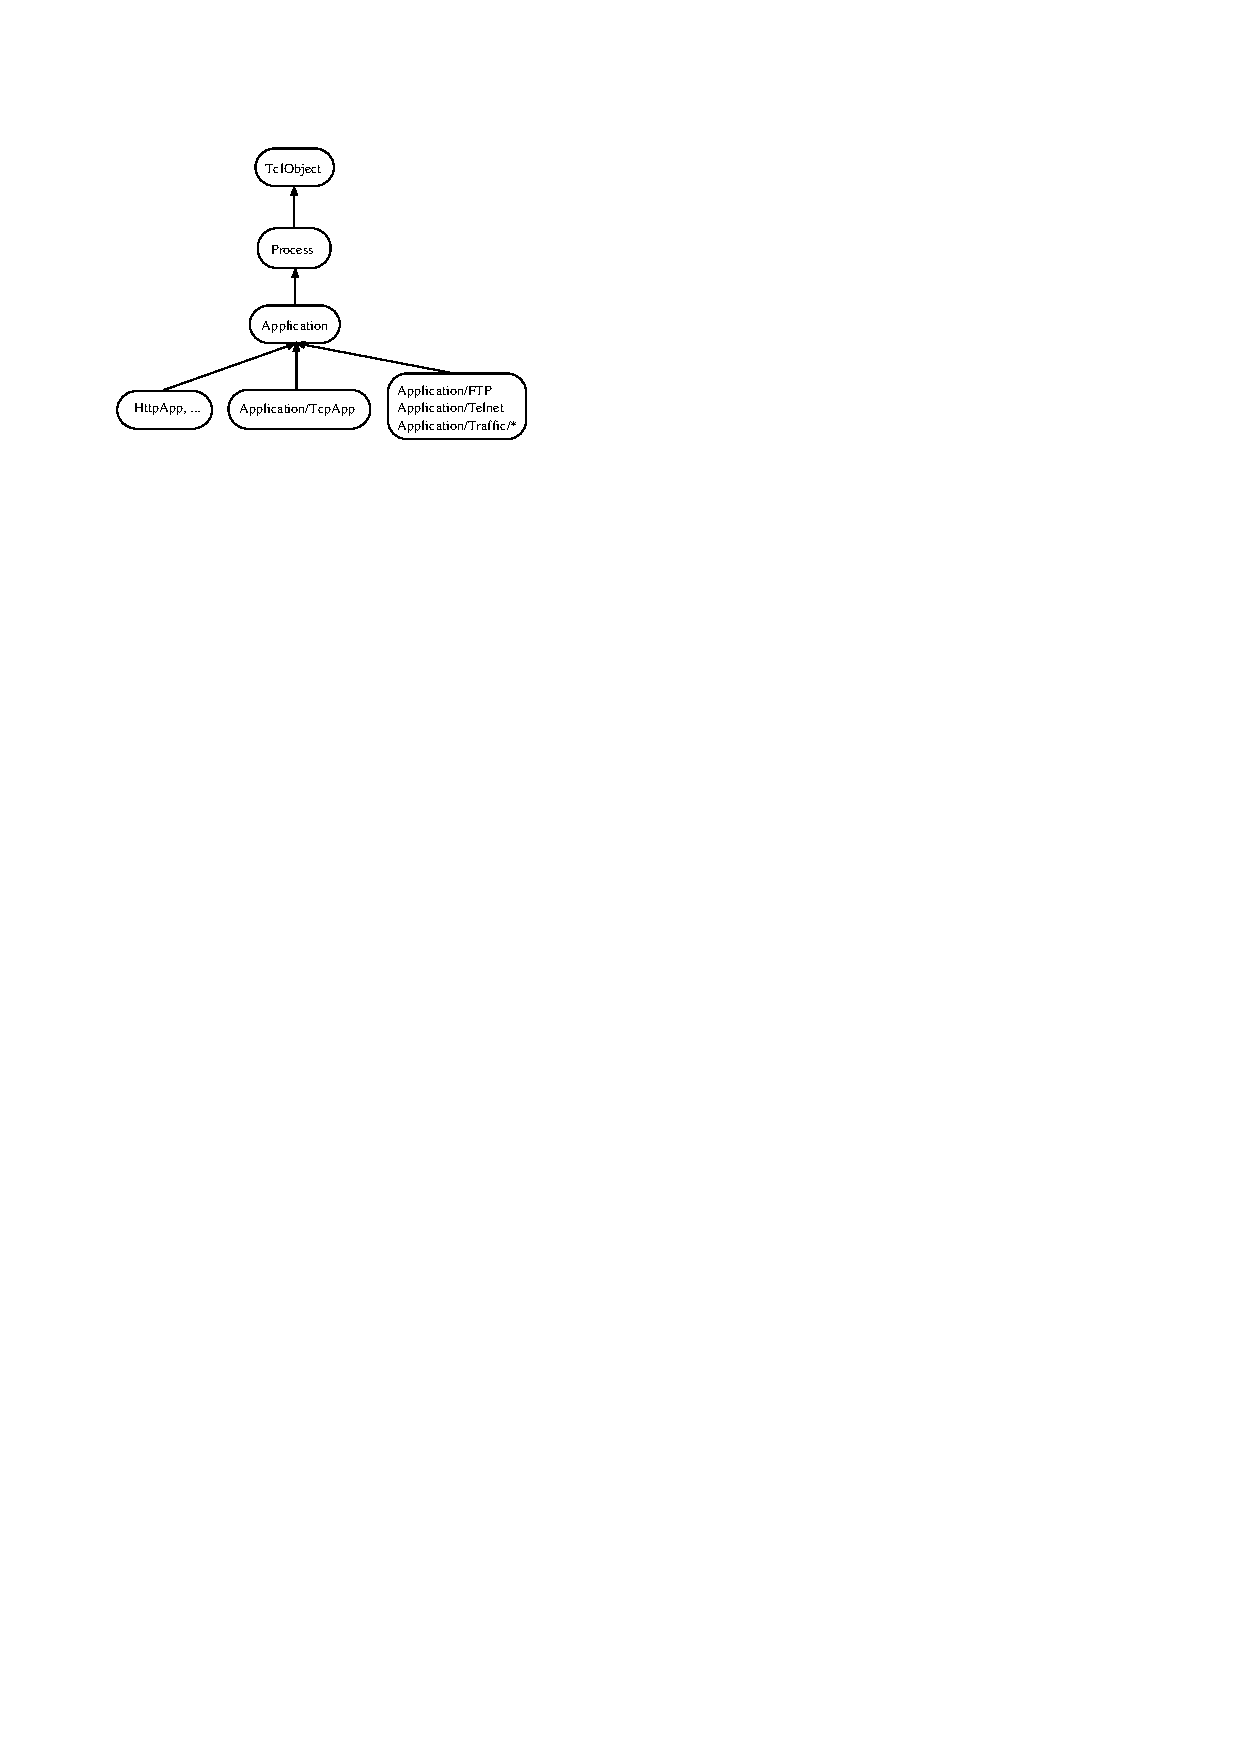
\includegraphics{appdata-hier}
    \caption{Hierarchy of classes related to application-level data handling}
    \label{fig:appdata-hier}
  \end{center}
\end{figure}


\section{Overview of web cache classes}
\label{sec:webcache-class}

There are three major classes related to web cache, as it is in the
real world: client (browser), server, and cache. Because they share a
common feature, i.e., the HTTP protocol, they are derived from the
same base class \code{Http} (Name of OTcl class, it's called
\code{HttpApp} in C++). For the following reasons, it's not a real
Application.  First, an HTTP object (i.e., client/cache/server) may
want to maintain multiple concurrent HTTP connections, but an
Application contains only one \code{agent_}.  Also, an HTTP object
needs to transmit real data (e.g., HTTP header) and that's provided by
TcpApp instead of any Agent. Therefore, we choose to use a standalone
class derived from TclObject for common features of all HTTP objects,
which are managing HTTP connections and a set of pages.  In the rest
of the section, we'll discuss these functionalities of Http. In the
next three sections, we'll in turn describe HTTP client, cache and
server.

\subsection{Managing HTTP connections}
\label{sec:webcache-connection}

Every HTTP connection is embodied as a TcpApp
object. Http maintains a hash of TcpApp objects, which are all of 
its active connections. It assumes that to any other Http, it 
has only one HTTP connection. It also allows dynamic establishment and 
teardown of connections. Only OTcl interface is provided for establishing,
tearing down a connection and sending data through a connection.

\paragraph{OTcl methods}
Following is a list of OTcl interfaces related to connection management 
in Http objects:

\begin{alist}
id & return the id of the Http object, which is the id of the node the object
is attached to. \\

get-cnc \tup{client} & return the TCP agent associated with \$client (Http object).\\

is-connected \tup{server} & return 0 if not connected to \$server, 1 otherwise.\\

send \tup{client} \tup{bytes} \tup{callback} & send \$bytes of data to 
\$client. When it's done, execute \$callback (a OTcl command). \\

connect \tup{client} \tup{TCP} & associate a TCP agent with \$client (Http object). That agent will be used to send packets \emph{to} \$client. \\

disconnect \tup{client} & delete the association of a TCP agent with \$client.
Note that neither the TCP agent nor \$client is not deleted, only the 
association is deleted.\\
\end{alist}

\paragraph{Configuration parameter}

By default, Http objects use Agent/SimpleTcp as transport agents
(section \ref{sec:webcache-tcpapp}). They can also use Agent/FullTcp
agents, which allows Http objects to operate in a lossy network.
Class variable code{TRANSPORT\_} is used for this purpose. E.g.,
\code{Http set TRANSPORT\_ FullTcp} tells all Http objects use
FullTcp agents.

This configuration should be done \emph{before} simulation starts, and 
it should not change during simulation, because FullTcp agents do not 
inter-operate with SimpleTcp agents.

\subsection{Managing web pages}
\label{sec:webcache-page}

Http also provides OTcl interfaces to manage a set of pages. The 
real management of pages are handled by class \code{PagePool} and its
subclasses. Because different HTTP objects have different requirements
for page management, we allow different PagePool subclasses to be attached
to different subclasses of Http class. Meanwhile, we export
a common set of PagePool interfaces to OTcl through
Http. For example, a browser may use a PagePool only to generate a 
request stream, so its PagePool only needs to contain a list of URLs. But
a cache may want to store page size, last modification time of every page 
instead of a list of URLs. However, this separation is not clearcut in 
the current implementation. 

Page URLs are represented in the form of:
\code{\tup{ServerName}:\tup{SequenceNumber}}
where the {\tt ServerName} is the name of OTcl object, and 
every page in every server should have a unique {\tt SequenceNumber}. 
Page contents are ignored. Instead, every page contains several 
\emph{attributes}, which are represented in OTcl as a list of the following 
(\tup{name} \tup{value}) pairs: ``modtime \tup{val}'' (page 
modification time), ``size \tup{val}'' (page size), and ``age \tup{val}''\}
The ordering of these pairs is not significant.

Following is a list of related OTcl methods.

\begin{alist}
set-pagepool \tup{pagepool} & set page pool \\

enter-page \tup{pageid} \tup{attributes} & add a page with id \$pageid
into pool. \$attributes is the attributes of \$pageid, as described above. \\

get-page \tup{pageid} & return page attributes in the format described 
above. \\

get-modtime \tup{pageid} & return the last modification time of the page 
\$pageid. \\

exist-page \tup{pageid} & return 0 if \$pageid doesn't exist in this 
Http object, 1 otherwise. \\

get-size \tup{pageid} & return the size of \$pageid. \\

get-cachetime \tup{pageid} & return the time when page \$pageid is entered
into the cache. \\
\end{alist}

\subsection{Debugging}
\label{sec:webcache-debug}

HttpApp provides two debugging methods. \code{log} registers a file 
handle as the trace file for all HttpApp-specific traces. Its trace format 
is described in section \ref{sec:webcache-trace}. \code{evTrace} logs a 
particular event into trace file. It concatenates
time and the id of the HttpApp to the given string, and writes it out. 
Details can be found in \ns/webcache/http.cc.


\section{Representing web pages}

We represent web pages as the abstract class Page. It is defined as follows:

\begin{program}
class Page \{
public:
        Page(int size) : size_(size) \{\}
        int size() const \{ return size_; \}
        int& id() \{ return id_; \}
        virtual WebPageType type() const = 0;

protected:
        int size_;
        int id_;
\};
\end{program}

It represents the basic properties of a web page: size and URL. Upon
it we derive two classes of web pages: ServerPage and ClientPage. The
former contains a list of page modification times, and is supposed to
by used by servers. It was originally designed to work with a special
web server trace; currently it is not widely used in \ns. The latter,
ClientPage, is the default web page for all page pools below. 

A ClientPage has the following major properties (we omit some
variables used by web cache with invalidation, which has too many
details to be covered here):

\begin{itemize}
\item \code{HttpApp* server_} - Pointer to the original server of this
  page. 
\item \code{double age_} - Lifetime of the page.
\item \code{int status_} - Status of the page. Its contents are
  explained below.
\end{itemize}

The status (32-bit) of a ClientPage is separated into two 16-bit
parts. The first part (with mask 0x00FF) is used to store page
status, the second part (with mask 0xFF00) is used to store expected
page actions to be performed by cache. Available page status are (again,
we omit those closely related to web cache invalidation):

\begin{alist}
HTTP\_VALID\_PAGE & Page is valid. \\
HTTP\_UNCACHEABLE & Page is uncacheable. This option can be used to
simulate CGI pages or dynamic server pages. \\
\end{alist}

CilentPage has the following major C++ methods: 

\begin{itemize}
\item \code{type()} - Returns the type of the page. Assuming pages of
  the same type should have identical operations, we let all
  ClientPage to be of type ``HTML''. If later on other types of web
  pages are needed, a class may be derived from ClientPage (or Page)
  with the desired type. 
\item \code{name(char *buf)} - Print the page's name into the given
  buffer. A page's name is in the format of:
  \tup{ServerName}:\tup{PageID}. 
\item \code{split_name(const char *name, PageID& id)} - Split a given
  page name into its two components. This is a static method. 
\item \code{mtime()} - Returns the last modification time of the page.
\item \code{age()} - Returns the lifetime of the page. 
\end{itemize}


\section{Page pools}
\label{sec:webcache-pagepool}

PagePool and its derived classes are used by servers to generate page
information (name, size, modification time, lifetime, etc.), by caches
to describe which pages are in storage, and by clients to generate a
request stream. Figure~\ref{fig:pagepool-hier} provides an overview of
the class hierarchy here. 

\begin{figure}[tb]
  \begin{center}
    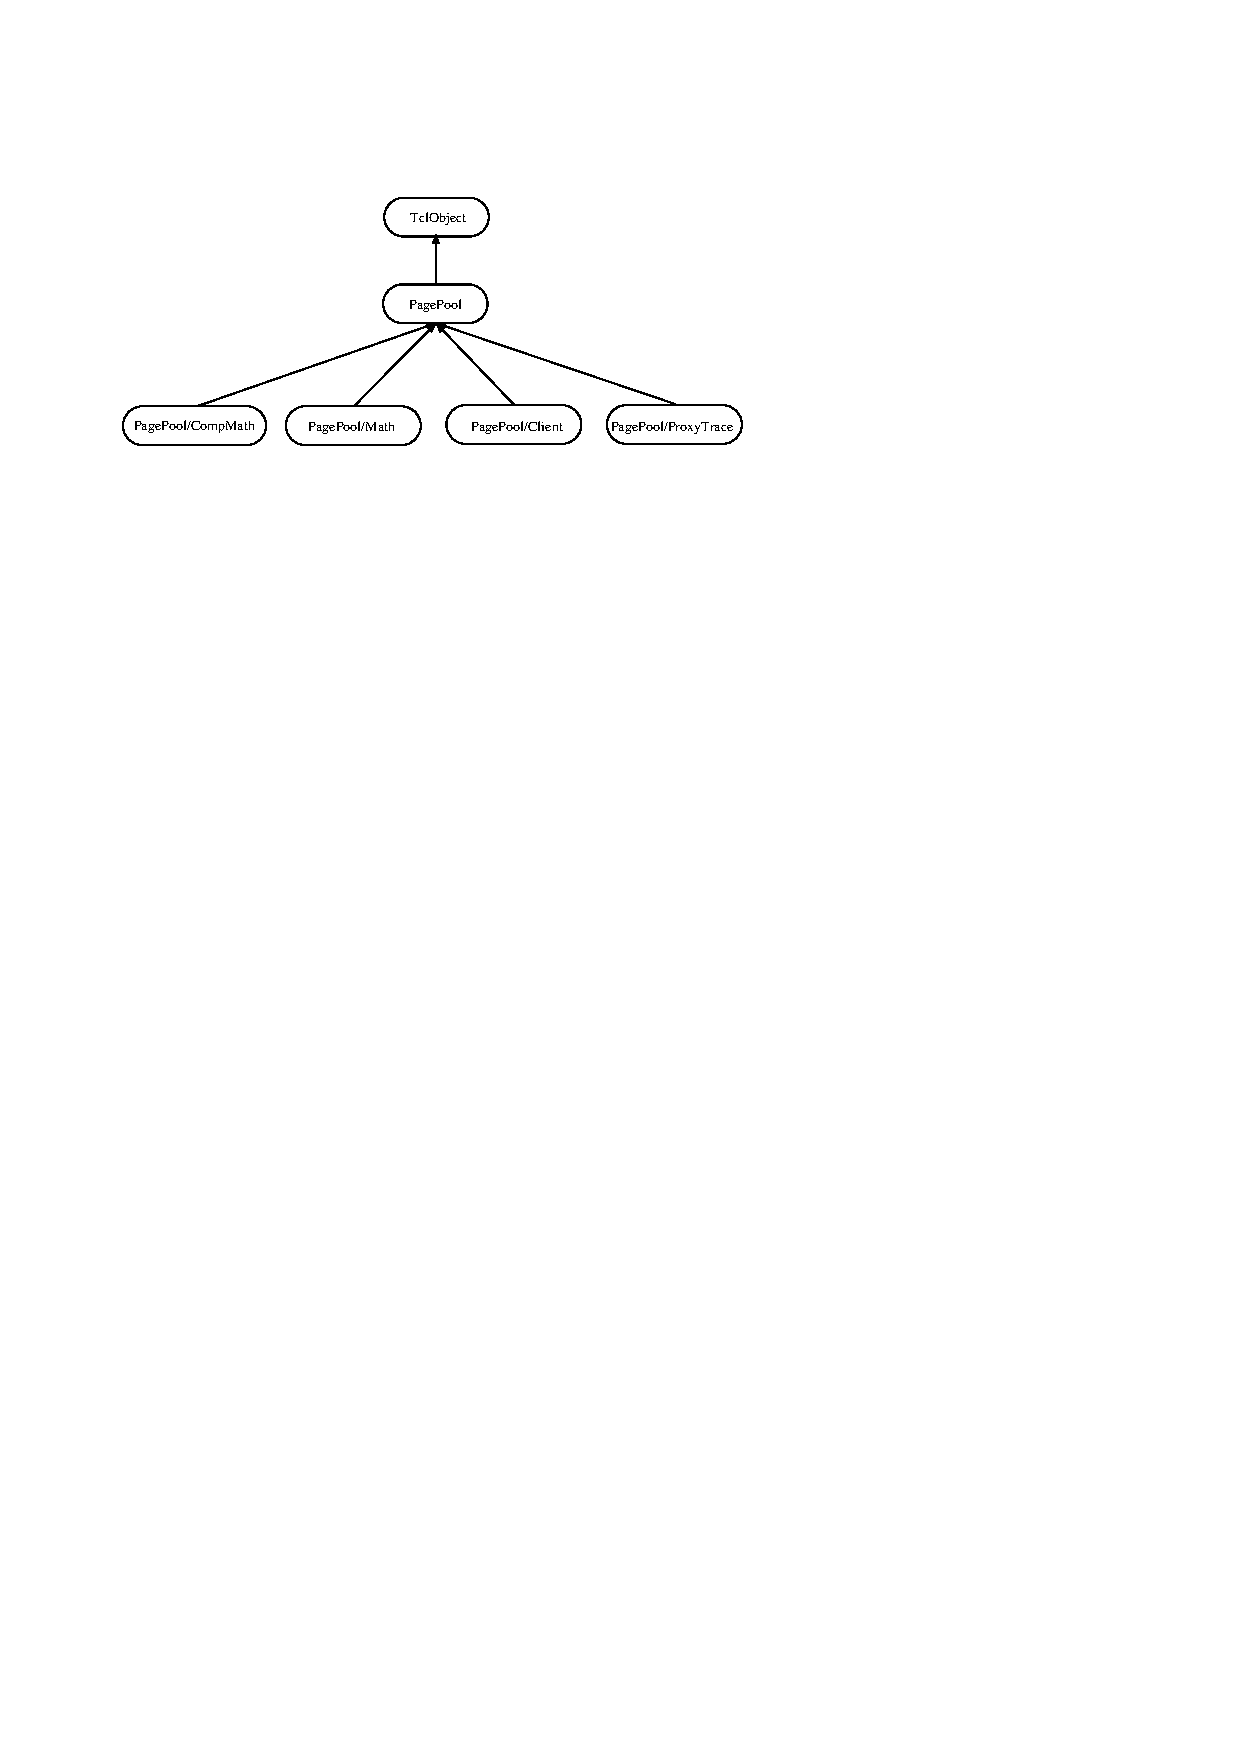
\includegraphics{pagepool-hier}
    \caption{Class hierarchy of page pools}
    \label{fig:pagepool-hier}
  \end{center}
\end{figure}

Among these, class PagePool/Client is mostly used by caches to store
pages and other cache-related information; other three classes are
used by servers and clients. In the following we describe these
classes one by one.

\subsection{PagePool/Math}

This is the simplest type of page pool. It has only one page, whose
size can be generated by a given random variable. Page modification
sequence and request sequence are 
generated using two given random variables. It has the following OTcl
methods:

\begin{alist}
gen-pageid & Returns the page ID which will be requested next. Because
 it has only one page, it always returns 0.\\

gen-size & Returns the size of the page. It can be generated by a
  given random variable. \\

gen-modtime \tup{pageID} \tup{mt} & Returns the next modification time of the
  page. \tup{mt} gives the last modification time. It uses the
  lifetime random variable. \\

ranvar-age \tup{rv} & Set the file lifetime random variable as
  \tup{rv}. \\

ranvar-size \tup{rv} & Set the file size random variable to be
  \tup{rv}. \\
\end{alist}

{\em NOTE}: There are two ways to generate a request sequence. With
all page pools except PagePool/ProxyTrace, request sequence is
generated with a random variable which describes the request
interval, and the \code{gen-pageid} method of other page pools gives
the page ID of the next request. PagePool/ProxyTrace loads the request
stream during initialization phase, so it does not need a random
variable for request interval; see its description below. 

An example of using PagePool/Math is at Section
\ref{sec:webcache-example}. That script is also available at 
\ns/tcl/ex/simple-webcache.tcl. 

\subsection{PagePool/CompMath}

It improves over PagePool/Math by introducing a compound page
model. By a compound page we mean a page which consists of a main text
page and a number of embedded objects, e.g., GIFs. We model a compound
page as a main page and several component objects. The main page is
always assigned with ID 0. All component pages
have the same size; both the main page size and component object size is
fixed, but adjustable through OTcl-bound variables \code{main_size_}
and \code{comp_size_}, respectively. The number of component objects
can be set using the OTcl-bound variable \code{num_pages_}.

PagePool/CompMath has the following major OTcl methods:

\begin{alist}
gen-size \tup{pageID} & If \tup{pageID} is 0, return
  \code{main\_size\_}, otherwise return \code{comp\_size\_}.\\

ranvar-main-age \tup{rv} & Set random variable for main page
  lifetime. Another one, \code{ranvar-obj-age}, set that for component
  objects. \\

gen-pageid & Always returns 0, which is the main page ID. \\ 

gen-modtime \tup{pageID} \tup{mt} & Returns the next modification time
  of the given page \tup{pageID}. If the given ID is 0, it uses the
  main page lifetime random variable; otherwise it uses the component
  object lifetime random variable. \\
\end{alist}

An example of using PagePool/CompMath is available at 
\ns/tcl/ex/simple-webcache-comp.tcl.

\subsection{PagePool/ProxyTrace}

The above two page pool synthesize request stream to a single web page
by two random variables: one for request interval, another for
requested page ID. Sometimes users may want more complicated request
stream, which consists of multiple pages and exhibits spatial locality
and temporal locality. There exists one proposal (SURGE
\cite{Barf98:WebWorkload}) 
which generates such request streams, we choose to provide an
alternative solution: use real web proxy cache trace (or server
trace). 

The class PagePool/ProxyTrace uses real traces to drive
simulation. Because there exist many web traces with different
formats, they should be converted into a intermediate format before
fed into this page pool. The converter is available at 
http://mash.cs.berkeley.edu/dist/vint/webcache-trace-conv.tar.gz.
It accepts four trace formats: DEC proxy trace (1996), UCB
Home-IP trace, NLANR proxy trace, and EPA web server trace. It
converts a given trace into two files: pglog and reqlog. Each line in
pglog has the following format:
\begin{center}
\begin{verbatim}
[<serverID> <URL_ID> <PageSize> <AccessCount>]
\end{verbatim}
\end{center}

Each line, except the last line, in reqlog has the following format:
\begin{center}
\begin{verbatim}
[<time> <clientID> <serverID> <URL_ID>]
\end{verbatim}
\end{center}

The last line in reqlog records the duration of the entire trace and
the total number of unique URLs:
\begin{center}
\begin{verbatim}
i <Duration> <Number_of_URL>
\end{verbatim}
\end{center}

PagePool/ProxyTrace takes these two file as input, and use them to
drive simulation. Because most existing web proxy traces do not
contain complete page modification information, we choose to use a
bimodal page modification model \cite{Cao97:CacheConsistency}. We
allow user to select $x\%$ of the pages to have one random page
modification interval generator, and the rest of the pages to have
another generator. In this way, it's possible to let $x\%$ pages to be
dynamic, i.e., modified frequently, and the rest static. Hot pages are
evenly distributed among all pages. For example, assume 10\% pages are
dynamic, then if we sort pages into a list according to their popularity,
then pages 0, 10, 20, $\ldots$ are dynamic, rest are static. Because
of this selection mechanism, we only allow bimodal ratio to change in
the unit of 10\%. 

In order to distribute requests to different requestors in the
simulator, PagePool/ProxyTrace maps the client ID in the traces to
requestors in the simulator using a modulo operation. 

PagePool/ProxyTrace has the following major OTcl methods:

\begin{alist}
get-poolsize & Returns the total number of pages. \\

get-duration & Returns the duration of the trace. \\

bimodal-ratio & Returns the bimodal ratio. \\

set-client-num \tup{num} & Set the number of requestors in the
simulation. \\

gen-request \tup{ClientID} & Generate the next request for the given
requestor. \\

gen-size \tup{PageID} & Returns the size of the given page. \\

bimodal-ratio \tup{ratio} & Set the dynamic pages to be \tup{ratio}*10
percent. Note that this ratio changes in unit of 10\%. \\

ranvar-dp \tup{ranvar} & Set page modification interval generator for 
dynamic pages. Similarly, ranvar-sp \tup{ranvar} sets the generator
for static pages. \\

set-reqfile \tup{file} & Set request stream file, as discussed
above. \\

set-pgfile \tup{file} & Set page information file, as discussed
above. \\

gen-modtime \tup{PageID} \tup{LastModTime} & Generate next
modification time for the given page. \\
\end{alist}

An example of using PagePool/ProxyTrace is available at 
\ns/tcl/ex/simple-webcache-trace.tcl. 


\subsection{PagePool/Client}

The class PagePool/Client helps caches to keep track of pages resident
in cache, and to store various cache-related information about
pages. It is mostly implemented in C++, because it is mainly used
internally and little functionality is needed by users. It has the
following major C++ methods:

\begin{itemize}
\item \code{get_page(const char* name)} - Returns a pointer to the
  page with the given name. 
\item \code{add_page(const char *name, int size, double mt, double et, double age)} - Add a page with given size, last modification
    time (mt), cache entry time (et), and page lifetime (age). 
\item \code{remove_page(const char* name)} - Remove a page from cache.
\end{itemize}

This page pool should support various cache replacement algorithms,
however, it has not been implemented yet. 

\subsection{PagePool/WebTraf}

The class PagePool/WebTraf is a standalone Web traffic modle that utilizes
PagePool framework. However, this class has nothing to do with the HttpApp 
classes. Because we are only interested in using it to study Web traffic 
pattern here, and do not want to be bothered with the burden of 
transmitting HTTP headers, etc. It has the following two major data structures.
Details can be found in ns/webcache/webtraf.cc and ns/webcache/webtraf.h, the
architecture WebTraf model is also loosely described in~\cite{Feldmann99a}, 
Section 2.4, paragraph 3-4 and the appendix A.1.

\begin{itemize}
\item \code{WebTrafSession} - a class that models Web user session. It is defined as follows:
\begin{program}
class WebTrafSession : public TimerHandler \{
	public:   
	        WebTrafSession(WebTrafPool *mgr, Node *src, int np, int id) : rvInterPage_(NULL),
	        rvPageSize_(NULL), rvInterObj_(NULL), rvObjSize_(NULL), mgr_(mgr), src_(src), 
	        nPage_(np), curPage_(0), donePage_(0), id_(id), interPageOption_(1) \{\} 
	        virtual ~WebTrafSession();

	        // Queried by individual pages/objects
	        inline RandomVariable*& interPage() \{ return rvInterPage_; \}
	        inline RandomVariable*& pageSize() \{ return rvPageSize_; \}
	        inline RandomVariable*& interObj() \{ return rvInterObj_; \}
	        inline RandomVariable*& objSize() \{ return rvObjSize_; \}
		
	        void donePage(void* ClntData); // all the pages within this
	                                       // session have  been sent
	        void launchReq(void* ClntData, int obj, int size);
	        inline int id() const \{ return id_; \}
	        inline WebTrafPool* mgr() \{ return mgr_; \}
	 private:
	        virtual void expire(Event *e = 0); // Lanuch request for a page
	        virtual void handle(Event *e); // schedule the timer for next page

	        RandomVariable *rvInterPage_, *rvPageSize_, *rvInterObj_, *rvObjSize_;
	        WebTrafPool* mgr_;
	        Node* src_;  // One Web client (source of request) per session
	        nt nPage_; // number of pages per session
	        int curPage_; // number of pages that have been sent
	        int id_; // page ID
	        int interPageOption_;
\}
\end{program}
\item \code{WebPage} - a class that models Web Page. It is defined as follows:
\begin{program}
class WebPage : public TimerHandler \{
	public:
	        WebPage(int id, WebTrafSession* sess, int nObj, Node* dst) :
	                id_(id), sess_(sess), nObj_(nObj), curObj_(0),
	                doneObj_(0), dst_(dst) \{\}
	        virtual ~WebPage() \{\}
	        inline void start() \{ // Call expire() and schedule the next one if needed     
	        void doneObject() \{ // All the objects within this page have been sent
	        inline int id() const \{ return id_; \}
	        Node* dst() \{ return dst_; \}
	        inline int curObj() const \{ return curObj_; \}
	        inline int doneObj() const \{ return doneObj_; \}
	private:  
	        virtual void expire(Event* = 0) \{ // Launch request for an object
	        virtual void handle(Event *e) \{ // schedule the timer for the next object
	        int id_; // object ID
	        WebTrafSession* sess_; // the session that requested this page
	        int nObj_; // number of object in this page
	        int curObj_ ; // number of object that have been sent
	        Node* dst_; //  server that this page has been requested from
\}
\end{program}
\end{itemize}

Following is a list of related OTcl methods to the WebTraf class.
\begin{alist}
set-num-session \tup{number-of-session} & set the total number of sessions in the WebTraf pool. \\
set-num-server \tup{number-of-server} & set the total number of servers. \\
set-num-client \tup{number-of-client} & set the total number clients. \\
set-interPageOption \tup{option} & There are two ways to interpret \emph{inter-page} time: One is the time between the start of two consecutive page downloads by the same user, and the other is the time between the end of previous page download and the start of the following page by the same user.  \$option can be set 
to either 0 or 1 (default is 1). When \$option is set to 1, the second interpretation is used for "inter-page" time. The first interpratation is adopted when \$option is set to 0. Note the resulted traffic volume using the first interpretation is much higher than the second interpretation. \\
doneObj \tup{webpage} & all the objects in \$webpage have been sent. \\
set-server \tup{id} \tup{node} & set \$node as server \$id. \\
set-client \tup{id} \tup{node} & set \$node as client \$id. \\
recycle \tup{tcp} \tup{sink} & Recycle a TCP source/sink pair. \\
create-session \tup{session-index} \tup{pages-per-sess} & \\
 \tup{launch-time} \tup{inter-page-rv} \tup{page-size-rv} & \\
 \tup{inter-obj-rv} \tup{obj-size-rv} & 
Create a Web session. \$session-index is the sesson index. \$pages-per-sess is
the total number of pages per session. \$launch-time is session starting time. 
\$inter-page-rv is the random variable that generates page inter-arrival time.
\$page-size-rv is the random variable that generates number of objects per page.
\$inter-obj-rv is the random variable that generates object inter-arrival time.
\$obj-size-rv is the random variable that generates object size. \\
\end{alist}

The example script is available at ns/tcl/ex/web-traffic.tcl (also
see ns/tcl/ex/large-scale-web-traffic.tcl for use of a large-scale web traffic 
simulation)

\section{Web client}
\label{sec:webcache-client}

Class Http/Client models behavior of a simple web browser. It
generates a sequence of page requests, where request interval and page 
IDs are randomized. It's a pure OTcl class inherited from Http. 
Next we'll walk through its functionalities and usage.

\paragraph{Creating a client}

First of all, we create a client and connect it to a cache and a web server.
Currently a client is only allowed to connect to a single cache, but it's 
allowed to connect to multiple servers. Note that this has to be called 
\emph{AFTER} the simulation starts (i.e., after \code{$ns run} %$
is called).
This remains true for all of the following methods and code examples of 
Http and its derived classes, unless explicitly said.

\begin{program}
        # Assuming $server is a configured Http/Server. 
        set client [new Http/Client $ns $node] \; client resides on this node;
        $client connect $server \; connecting client to server;
\end{program} %$

\paragraph{Configuring request generation}

For every request, Http/Client uses PagePool to generate a random page
ID, and use a random variable to generate intervals between two 
consecutive requests:
\footnote{Some PagePool,
e.g., PagePool/Math, has only one page and therefore it always returns the
same page. Some other PagePool, e.g. PagePool/Trace, has multiple pages 
and needs a random variable to pick out a random page.} 

\begin{program}
        $client set-page-generator $pgp \; attach a configured PagePool;
        $client set-interval-generator $ranvar \; attach a random variable;
\end{program}

Here we assume that PagePools of Http/Client share the same set of pages
as PagePools of the server. Usually we simplify our simulation by letting
all clients and servers share the same PagePool, i.e., they have the same
set of pages. When there are multiple servers, or servers' PagePools 
are separated from those of clients', care must be taken to make sure that 
every client sees the same set of pages as the servers to which they are
attached.

\paragraph{Starting}

After the above setup, starting requests is very simple:

\begin{program}
        $client start-session $cache $server \; assuming $cache is a configured Http/Cache;
\end{program}

\paragraph{OTcl interfaces}
Following is a list of its OTcl methods (in addition to those
inherited from Http). This is not a complete list. More details can be
found in \ns/tcl/webcache/http-agent.tcl.

\begin{alist}
send-request \tup{server} \tup{type} \tup{pageid} \tup{args} & 
send a request of page \$pageid and type \$type to \$server. The only 
request type allowed for a client is GET. \$args has a format identical
to that of \$attributes described in \code{Http::enter-page}. \\

start-session \tup{cache} \tup{server} & start sending requests of a 
random page to \$server via \$cache. \\

start \tup{cache} \tup{server} & before sending requests, populate
\$cache with all pages in the client's PagePool. This method is useful 
when assuming infinite-sized caches and we want to observe behaviors 
of cache consistency algorithms in steady state. \\

set-page-generator \tup{pagepool} & attach a PagePool to generate 
random page IDs.\\

set-interval-generator \tup{ranvar} & attach a random variable to generate
random request intervals.\\
\end{alist}


\section{Web server}
\label{seccom:webcache-server}

Class Http/Server models behavior of a HTTP server. Its
configuration is very simple. All that a user needs to do is to create 
a server, attach a PagePool and wait:

\begin{program}
        set server [new Http/Server $ns $node] \; attach \$server to \$node;
        $server set-page-generator $pgp \; attach a page pool;
\end{program}

An Http/Server object waits for incoming requests after simulation starts.
Usually clients and caches initiates connection to an Http/Server. But 
it still has its own \code{connect} method, which allows an Http/Server 
object to actively connect to a certain cache (or client). Sometimes this
is useful, as explained in Test/TLC1::set-groups\{\} in 
\ns/tcl/test/test-suite-webcache.tcl.

An Http/Server object accepts two types of requests: GET and IMS.  GET
request models normal client requests. For every GET request, it
returns the attributes of the requested page.  IMS request models
If-Modified-Since used by TTL algorithms for cache consistency. For
every IMS (If-Modified-Since) request, it compares the page
modification time given in the request and that of the page in its
PagePool. If the time indicated in the request is older, it sends back
a response with very small size, otherwise it returns all of the page 
attributes with response size equal the real page size.


\section{Web cache}
\label{sec:webcache-cache}

Currently 6 types of web caches are implemented, including 
the base class Http/Cache. Its five derived subclasses 
implement 5 types of cache consistency algorithms: Plain old TTL, 
adaptive TTL, Omniscient TTL, Hierarchical multicast invalidation, 
and hierarchical multicast invalidation plus direct request.

In the following we'll only describe the base class Http/Cache, because 
all the subclasses involves discussion of cache consistency algorithms 
and it does not seem to be appropriate here.

\subsection{Http/Cache}
\label{sec:webcache-cache-base}

Class Http/Cache models behavior of a simple HTTP cache with infinite 
size. It doesn't contain removal algorithm, nor consistency algorithm. 
It is not intended to be used by itself. Rather, it is meant to be a 
base class for experimenting with various cache consistency algorithms and
other cache algorithms. 

\paragraph{Creation and startup}

Creating an Http/Cache requires the same set of parameters as
Http/Client and Http/Server. After creation, a cache needs to connect 
to a certain server. Note that this creation can also be done dynamically,
when a request comes in and the cache finds that it's not connected to 
the server. However, we do not model this behavior in current code.
Following code is an example:

\begin{program}
        set cache [new HttpCache $ns $node] \; attach cache to \$node;
        $cache connect $server \; connect to \$server;
\end{program}

Like Http/Server, an Http/Cache object waits for requests (and packets
from server) after it's initialized as above. When hierarchical
caching is used, the following can be used to create the hierarchy:

\begin{program}
        $cache set-parent $parent \; set parent cache;
\end{program}

Currently all TTL and multicast invalidation caches support hierarchical
caching. However, only the two multicast invalidation caches allows 
multiple cache hierarchies to inter-operate.

\paragraph{OTcl methods}

Although Http/Cache is a SplitObject, all of its methods are in OTcl. 
Most of them are used to process an incoming request. Their relations can
be illustrated with the flowchart below, followed by explainations:

\begin{figure}[h]
  \begin{center}
    \includegraphics{cache-flowchart}
    \caption{Handling of incoming request in Http/Cache}
    \label{fig:webcache-handle-request}
  \end{center}
\end{figure}

\begin{alist}
get-request \tup{client} \tup{type} \tup{pageid} & 
The entry point of processing any request. It checks if the requested 
page \$pageid exists in the cache's page pool, then call either 
\code{cache-hit} or \code{cache-miss}. \\

cache-miss \tup{client} \tup{type} \tup{pageid} & 
This cache doesn't have the page. Send a request to server (or parent 
cache) to refetch the page if it hasn't already done so. Register 
\$client in a list so that when the cache gets the page, it'll forward
the page to all clients who have requested the page. \\

cache-hit \tup{client} \tup{type} \tup{pageid} &
Checks the validatity of the cached page. If it's valid, send \$client
the cached page, otherwise refetch the page. \\ 

is-consistent \tup{client} \tup{type} \tup{pageid} & 
Returns 1 if \$pageid is valid. This is intended to be overridden by 
subclasses. \\

refetch \tup{client} \tup{type} \tup{pageid} & 
Refetch an invalid page from server. This is intended to be overridden 
by subclasses. \\
\end{alist}


\section{Putting together: a simple example}
\label{sec:webcache-example}

We have seen all the pieces, now we present a script which provides a
complete view of all pieces together. First, we build topology and 
other usual initializations:

\begin{program}
        set ns [new Simulator]

        # Create topology/routing
        set node(c) [$ns node] 
        set node(e) [$ns node]
        set node(s) [$ns node]
        $ns duplex-link $node(s) $node(e) 1.5Mb 50ms DropTail
        $ns duplex-link $node(e) $node(c) 10Mb 2ms DropTail 
        $ns rtproto Session
\end{program}

Next we create the Http objects:

\begin{program}
        # HTTP logs
        set log [open "http.log" w]

        # Create page pool as a central page generator. Use PagePool/Math
        set pgp [new PagePool/Math]
        set tmp [new RandomVariable/Constant] \;# Page size generator;
        $tmp set val_ 1024  \;# average page size;
        $pgp ranvar-size $tmp
        set tmp [new RandomVariable/Exponential] \;# Page age generator;
        $tmp set avg_ 5 \;# average page age;
        $pgp ranvar-age $tmp

        set server [new Http/Server $ns $node(s)] \;# Create a server and link it to the central page pool;
        $server set-page-generator $pgp
        $server log $log

        set cache [new Http/Cache $ns $node(e)] \;# Create a cache;
        $cache log $log

        set client [new Http/Client $ns $node(c)] \;# Create a client;
        set tmp [new RandomVariable/Exponential] \;# Poisson process as request sequence;
        $tmp set avg_ 5 \;# average request interval;
        $client set-interval-generator $tmp
        $client set-page-generator $pgp
        $client log $log

        set startTime 1 \;# simulation start time;
        set finishTime 50 \;# simulation end time;
        $ns at $startTime "start-connection"
        $ns at $finishTime "finish"
\end{program} %$

Then we define a procedure which will be called after simulation
starts.  The procedure will setup connections among all Http objects.
\begin{program}
        proc start-connection \{\} \{
                global ns server cache client
                $client connect $cache
                $cache connect $server
                $client start-session $cache $server
        \}
\end{program} %$

At the end, the usual closing:
\begin{program}
        proc finish \{\} \{
                global ns log
                $ns flush-trace
                flush $log
                close $log
                exit 0
        \}
        $ns run
\end{program}

This script is also available at \ns/tcl/ex/simple-webcache.tcl. 
Examining its output \code{http.log}, one will find that the result of 
the absense cache consistency algorithm results in a lot of stale hits. 
This can be easily remedied by replacing ``new Http/Cache'' line with:
\code{set cache [new Http/Cache/TTL $ns $node(e)]}. For more complicated
cache consistency algorithm examples, see 
\ns/tcl/test/test-suite-webcache.tcl.

\section{Http trace format}
\label{sec:webcache-trace}

The trace file of Http agents are constructed in a similar way as the
SRM trace files. It consists of multiple entries, each of which
occupies one line.  The format of each entry is:

\begin{tabular}[h]{c|c|c}
  Time & ObjectID & Object Values
\end{tabular}

There are three types of objects: client ({\bf C}), cache ({\bf E})
and server ({\bf S}). Following is a complete enumeration of all possible 
events and value types associated with these three types of objects.

\begin{center}
  \begin{tabular}[h]{c|c|l}
    \emph{Object Type} & \emph{Event Type} & \emph{Values} \\ \hline
    E & HIT & \tup{Prefix} \\
    E & MISS & \tup{Prefix} z \tup{RequestSize} \\
    E & IMS & \tup{Prefix} z \tup{Size} t \tup{CacheEntryTime} \\
    E & REF & p \tup{PageID} s \tup{ServerID} z \tup{Size} \\
    E & UPD & p \tup{PageID} m \tup{LastModifiedTime} z \tup{PageSize} \\
    &     & s \tup{ServerID} \\ 
    E & GUPD & z \tup{PageSize} \\
    E & SINV & p \tup{PageID} m \tup{LastModTime} z \tup{PageSize} \\
    E & GINV & p \tup{PageID} m \tup{LastModTime} \\
    E & SPF & p \tup{PageID} c \tup{DestCache} \\
    E & RPF & p \tup{PageID} c \tup{SrcCache} \\
    E & ENT & p \tup{PageID} m \tup{LastModifiedTime} z \tup{PageSize} \\
    &     & s \tup{ServerID} \\ \hline
    C & GET & p \tup{PageID} s \tup{PageServerID} z \tup{RequestSize}\\
    C & STA & p \tup{PageID} s \tup{OrigServerID} l \tup{StaleTime}\\
    C & RCV & p \tup{PageID} s \tup{PageServerID} l \tup{ResponseTime} z \tup{PageSize}\\ \hline
    S & INV & p \tup{PageID} m \tup{LastModifiedTime} z \tup{Size} \\
    S & UPD & p \tup{PageID} m \tup{LastModifiedTime} z \tup{Size} \\
    S & SND & p \tup{PageID} m \tup{LastModifiedTime} z \tup{PageSize} \\
      &     & t \tup{Requesttype} \\
    S & MOD & p \tup{PageID} n \tup{NextModifyTime} \\
  \end{tabular}
\end{center}

\tup{Prefix} is the information common to all trace entries. It includes:

\begin{center}
  \begin{tabular}[h]{c|c|c}
    p \tup{PageID} & c \tup{RequestClientID} & s \tup{PageServerID}
  \end{tabular}
\end{center}

\emph{Short Explaination of event operations}: 

\begin{center}
  \begin{tabular}[h]{c|c|l}
    \emph{Object Type} & \emph{Event Type} & \emph{Explaination} \\ \hline
    E & HIT & Cache hit. PageSererID is the id of the ``owner'' of the page. \\
    E & MISS & Cache miss. In this case the cache will send a request to the
    server to fetch the page. \\
    E & IMS & If-Modified-Since. Used by TTL procotols to validate an expired 
    page. \\
    E & REF & Page refetch. Used by invalidation protocols to refetch an 
    invalidated page. \\
    E & UPD & Page update. Used by invalidation protocols to ``push'' updates\\
      & & from parent cache to children caches. \\
    E & SINV & Send invalidation. \\
    E & GINV & Get invalidation. \\
    E & SPF & Send a pro forma \\
    E & RPF & Receive a pro forma \\
    E & ENT & Enter a page into local page cache. \\ 
    \hline
    C & GET & Client sends a request for a page. \\
    C & STA & Client gets a stale hit. OrigModTime is the modification time \\
    & & in the web server, CurrModTime is the local page's modification time.\\
    C & RCV & Client receives a page. \\
    \hline
    S & SND & Server send a response. \\
    S & UPD & Server pushes a page update to its ``primary cache''. Used by
    invalidation protocol only. \\
    S & INV & Server sends an invalidation message. Used by invalidation 
    protocol only. \\
    S & MOD & Server modified a page. The page will be modified next
    at \tup{NextModifyTime}. \\
  \end{tabular}
\end{center}


\section{Commands at a glance}
\label{sec:webcachecommand}

Following are the web cache related commands:
\begin{flushleft}
\code{set server [new Http/Server <sim> <s-node>]}\\
This creates an instance of an Http server at the specified <s-node>. An
instance of the simulator <sim> needs to be passed as an argument.


\code{set client [new Http/Client <sim> <c-node>]}\\
This creates an instance of a Http client at the given <c-node>.


\code{set cache [new Http/Cache <sim> <e-node>}\\
This command creates a cache.


\code{set pgp [new PagePool/<type-of-pagepool>]}\\
This creates a pagepool of the type specified. The different types of pagepool
currently implemented are:\\
PagePool/Math, PagePool/CompMath, PagePool/ProxyTrace and PagePool/Client.
See section \ref{sec:webcache-pagepool} for details on Otcl interface for
each type of Pagepool.


\code{$server set-page-generator <pgp>}\\
\code{$server log <handle-to-log-file>}\\
The above commands consist of server configuration. First the server is
attached to a central page pool <pgp>. Next it is attached to a log file.


\begin{program}
client set-page-generator <pgp>
$client set-interval-generator <ranvar> 
$client log <handle-to-log-file>
\end{program}
These consist configuration of the Http client. It is attached to a central
page pool <pgp>. Next a random variable <ranvar> is attached to the client
that is used by it (client) to generate intervals between two consecutive
requests. Lastly the client is attached to a log file for logging its events.


\code{$cache log <log-file>}\\
This is part of cache configuration that allows the cache to log its
events in a log-file. 


\code{$client connect <cache>}\\
\code{$cache connect <server>}\\
Once the client, cache, and server are configured, they need to be
connected as shown in above commands.


\code{$client start-session <cache> <server>}\\
This starts sending request for a random page from the client to the
<server> via <cache>.

\end{flushleft}
\endinput

% Local Variables:
% TeX-master: "everything"
% LocalWords:
% End:
% LocalWords:  HTTP tb app dataflow ADU OTcl AppData AppDataType struct hdr buf
% LocalWords:  const AppConnector inline int TclCL HttpApp webcache http nbytes
% LocalWords:  userdata HttpInvalAgent inteded inval recv realsize inv FullTcp
% LocalWords:  SimpleTcp bi str dsize Tcl tcl tcp iss ns TcpApps Mb ms DropTail
% LocalWords:  tmp val RandomVariable pgp ranvar avg startTime finishTime proc
